%\pgfdeclarelayer{background}
%\pgfdeclarelayer{foreground}
%\pgfsetlayers{background,main,foreground}

\pgfplotsset{
	axis background/.style={fill=none},
	%tick style=mygrey2,
	%tick label style=mygrey2,
	grid=none,
	%xtick pos=left,
	%ytick pos=left,
	tick style={
		major grid style={style=white,line width=1pt},minor grid style=white,
%		major grid style={style=white,line width=1pt},minor grid style=mygrey3,
		%tick align=outside,
	},
	%minor tick num=4,
}

\begin{figure}[tb]
	\centering
	 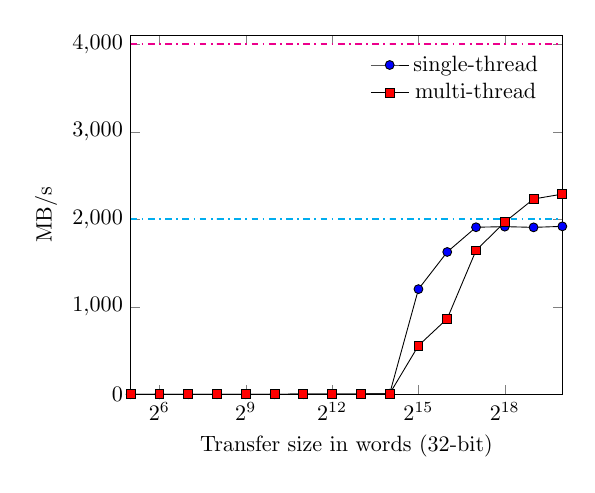
\begin{tikzpicture}[scale = 0.8]
	 \begin{axis}[
	 xmode=log,
	 log basis x={2},
	 xlabel=Transfer size in words (32-bit),
	 ymin=0,
	 ymax=4100,
	 xmax = 1048576,
	 xmin = 32,
	 ylabel=MB/s,
%	 legend style={at={(0.3,0.8)},anchor=north}
	 legend pos=north east,
	 legend style={draw=none}
	 ]    

	\addplot [mark=*,mark options={fill=blue}] plot coordinates {
		(32,     0)
		(64,     0)
		(128,    0.05)
		(256,     0.1)
		(512,      0.2)
		(1024,     0.35)
		(2048,     0.7)
		(4096,     1.45)
		(8192,     2.9)
		(16384,    5.85)
		(32768,    1201.5)
		(65536,    1626.5)
		(131072,   1909.1)
		(262144,   1915.8)
		(524288,   1907.7)
		(1048576,  1919.1)	
	}; 
	 \addplot [mark=square*,mark options={fill=red}] plot coordinates {
	 	(32,     0)
	 	(64,     0)
	 	(128,    0.04)
	 	(256,    0.08)
	 	(512,    0.16)
	 	(1024,   0.32)
	 	(2048,   0.68)
	 	(4096,   1.36)
	 	(8192,   2.76)
	 	(16384,  5.85)
	 	(32768,  556)
	 	(65536,  864)
	 	(131072, 1644)
	 	(262144, 1968)
	 	(524288, 2232)
	 	(1048576, 2288)
	 }; 
	 \addplot [color=cyan,thick,dash dot] plot coordinates {
	 	(32,     2000)
		(64,     2000)
		(128,     2000)
		(256,     2000)
		(512,     2000)
		(1024,     2000)
		(2048,     2000)
		(4096,     2000)
		(8192,     2000)
		(16384,    2000)
		(32768,    2000)
		(65536,    2000)
		(131072,    2000)
		(262144,    2000)
		(524288,    2000)
		(1048576,   2000)	
	 };

	 \addplot [color=magenta,thick,dash dot] plot coordinates {
	(32,     4000)
	(64,     4000)
	(128,     4000)
	(256,     4000)
	(512,     4000)
	(1024,     4000)
	(2048,     4000)
	(4096,     4000)
	(8192,     4000)
	(16384,    4000)
	(32768,    4000)
	(65536,    4000)
	(131072,   4000)
	(262144,   4000)
	(524288,   4000)
	(1048576,  4000)	
};

	 \legend{single-thread\\multi-thread\\}
	 \end{axis}
	 \end{tikzpicture}	
	
	\caption[]{PCIe-Xillybus loopback throughput.} 
	\label{pcie_xillybus_loopback_bw}
	
\end{figure}
